\chapter{Softwaredesign}

\section*{Version}
\begin{table}[h]
	\centering
	\begin{tabularx}{\textwidth - 2cm}{|l|l|l|X|}
	\hline
	Dato			& Version		& Initialer 	& Ændring																	\\ \hline
	23. November	& 1 			& Alle			& Første udkast. 															\\ \hline
	03. December 	& 2 			& PKP			& Opdateret data-klasse beskrivelse og tilføjet log-klasse beskrivelse. 	\\ \hline
	08. December 	& 3 			& KE			& Tilføjet Psoc-klasse (pi) 											\\ \hline
	10. december 	& 4 			& LS			& Tilføjet PSoC (psoc) samt opdateret sekvens diagrammer.					\\ \hline
\end{tabularx}
\end{table}
\clearpage

\section{Bil}

\subsection{Diagrammer for bil}

\subsubsection{BDD for bil} % bdd_bil.pdf

Dette diagram viser blokken bil fra figur \ref{fig:bdd_au2}. Blokken 'bil' skal forstås som alle mekaniske og elektriske som er fastgjort på køretøjet. Således er 

\begin{figure}[h]
\centering
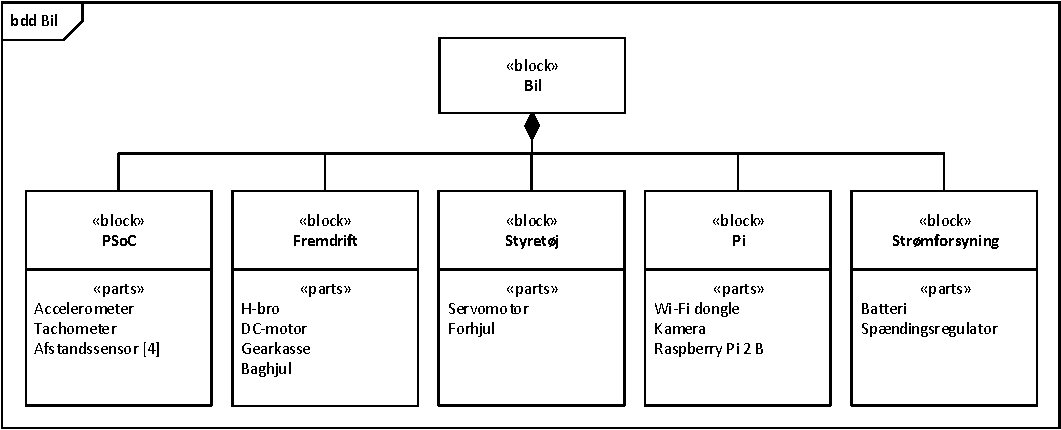
\includegraphics[width=\textwidth]{../fig/diagrammer/bil/bdd_bil.pdf}
\caption{BDD for bil}
\label{fig:bdd_bil}
\end{figure}
\clearpage

\subsubsection{IBD for signaler i bil}

På figur \ref{fig:ibd_bil} ses de interne forbindelser for figur \ref{fig:bdd_bil}. Diagrammet skaber et overblik over hvilke signaler der sendes og modtages. Bemærk at alle forsyningerne ikke er taget med på diagrammet, men istedet er lavet i et diagram for sig. Forsyningerne kan ses på figur \ref{fig:ibd_bil_forsyning}.

\begin{figure}[h]
\centering
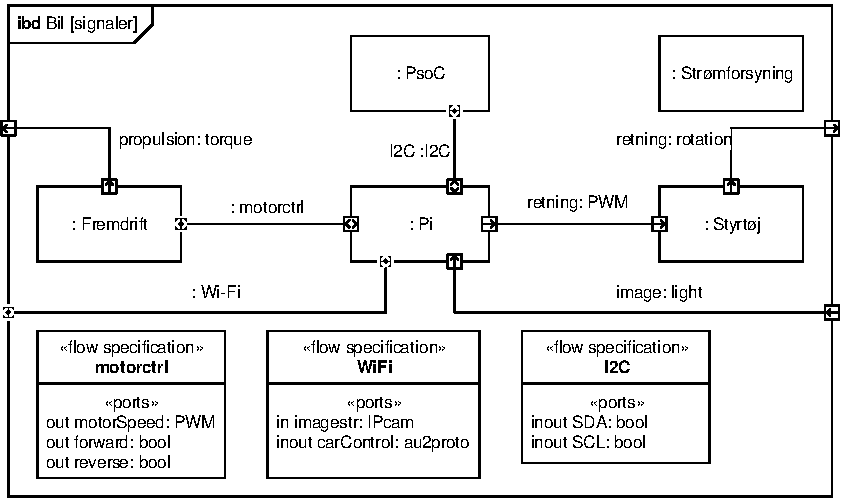
\includegraphics[scale=1]{../fig/diagrammer/bil/ibd_bil.pdf}
\caption{IBD for bil}
\label{fig:ibd_bil}
\end{figure}

\clearpage
\subsubsection{Signalbeskrivelser for bilens signaler}

\begin{table}[h]
	\centering
	\begin{tabularx}{\textwidth}{|l|Z|Z|Z|} \hline
	\textbf{Signal (navn: type)} & \textbf{Funktion} & \textbf{Tolerancer} & \textbf{Kommentarer} \\ \hline

Propulsion: torque
	& Baghjulenes torque til underlaget.
	& ~
	& ~
	\\ \hline

motorSpeed: PWM
	& Et PWM signal der bestemmer motorhastigheden. 
	& Frekvens: 30kHz +/- 1kHz 0-5V +/- 0.2V
 	& Logisk signal: \newline
		Lav = 0V +/- 0.2V \newline
		Høj = 5V +/- 0.2V
	\\ \hline

forward: bool
	& Kontrolsignal til H-bro.
	& 0-5V $\pm$ 0.2V
	& Lav = 0V +/- 0.2V  ’idle’ \newline
		Høj =  5V +/- 0.2V  ’frem’
	\\ \hline
	
reverse: bool
	& Kontrolsignal til H-bro.
	& 0-5V $\pm$ 0.2V
	& Lav = 0V +/- 0.2V ’idle’ \newline
		Høj =  5V +/- 0.2V  ’tilbage’
	\\ \hline
	
Inout SDA: bool
	& \IIC dataline til sensorer herunder accelerometer og afstandssensorer. 
	& 0-5V $\pm$ 0.5V
 	& Logisk signal: \newline
		Lav = 0V $\pm$ 0.5V \newline
		Høj = 7.2V $\pm$ 0.5V
	\\ \hline

Inout SCL: bool
	& \IIC clockline  til sensorer herunder accelerometer og afstandssensorer. 
	& 0-5V $\pm$ 0.5V
 	& Logisk signal: \newline
		Lav = 0V $\pm$ 0.5V \newline
		Høj = 7.2V $\pm$ 0.5V
	\\ \hline

Pulses: sound
	& Ultralydsbølger afsendt af sensor. 
	& Jfv. Datablad (henvisning kommer senere) %TODO henvsining
 	& ~
	\\ \hline
	
reflection: sound
	& Refleksionsbølge af udsendte ultralydsbølger. 
	& Jfv. Datablad (henvisning kommer senere) %TODO henvsining
 	& ~
	\\ \hline
	
retning: PWM 
	& PWM signal der vha pulsbredden angiver hvilken retning servomotoren skal 				dreje og dermed hvilken retning bilen skal dreje. 
	& Pulsbredde: 0.5ms – 2.5ms \newline
		Freq = 360Hz \newline
		0.5ms = 18\% Duty cycle (Venstre)\newline
		2.5ms = 90\% Duty cycle (Højre)
	& ~
	\\ \hline

retning: rotation
	& Får bilen til at dreje.
	& 30 grader til hhv. venstre og højre $\pm$ 5 grader
	& ~
	\\ \hline
	
imagestr: IPcam
	& Karsten... Hej%TODO Karsten 
	& ~ 
	& ~
	\\ \hline

carControl: au2proto
	& Få fingeren ud. %TODO Karsten
	& ~
	& ~
	\\ \hline

	\end{tabularx}
	\label{tbl:bil_signaler}
\end{table}

\clearpage

\subsubsection{Forsyninger} % ibd_bil_forsyning.pdf

Diagrammet på figur \ref{fig:ibd_bil_forsyning} tilsvarer direkte figur \ref{fig:ibd_bil}, blot med beskrivelsen af forsyning. Dette giver forbedret overblik da de to diagrammer sat sammen bliver uoverskueligt.  

\begin{figure}[h]
\centering
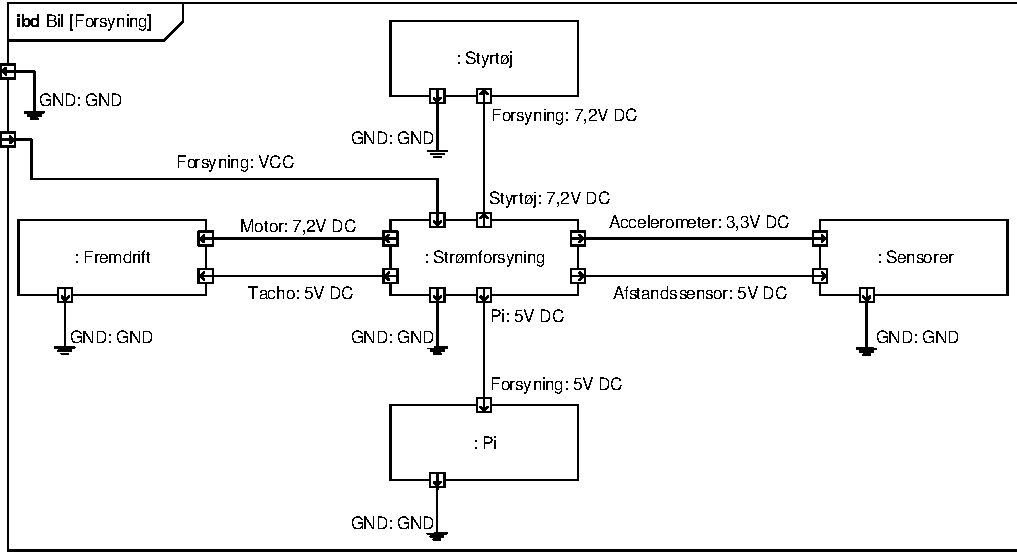
\includegraphics[width=\textwidth]{../fig/diagrammer/bil/ibd_bil_forsyning.pdf}
\caption{IBD for bilens forsyninger}
\label{fig:ibd_bil_forsyning}
\end{figure}

\clearpage

\subsubsection{Signalbeskrivelse for bilens forsyning}

\begin{table}[h]
	\centering
	\begin{tabularx}{\textwidth}{|l|Z|Z|Z|} \hline
	\textbf{Signal (navn: type)} & \textbf{Funktion} & \textbf{Tolerancer} & \textbf{Kommentarer} \\ \hline
forsyning: VCC
	& Forsyningsspænding fra det tilkoblede batteri. 
	& 7.2V DC $\pm$ 1V max. 20A
 	& Aflæst på batteriet.
	\\ \hline
	
GND: GND
	& Reference. 
	& 0V
 	& ~
	\\ \hline
	
styrtøj: 7.2V DC
	& Forsyningsspænding til styrtøj herunder servomotor. 
	& 7.2V DC $\pm$ 0,5V max 400 mA
 	& Fundet i databladet for servoen \cite{lib:servo}.
	\\ \hline
	
Psoc: 5V DC
	& Forsyningsspænding til Psoc. 
	& 5V DC $\pm$ 0,5V max 500 mA
 	& Worst case vurdering på baggrund af USB forsyning fra PC.
	\\ \hline
	
	
accelerometer: 3.3V DC
	& Forsyningsspænding til accelerometeret.
	& 3.3V DC $\pm$ 0.2V max 8 mA
 	& Fundet i databladet for servoen \cite{lib:accel}.
	\\ \hline
	
afstandssensor: 5V DC
	& Individuel forsyningsspænding til afstandssensorerne.
	& 5V DC $\pm$ 0.5V max 400 mA
 	& Fundet i databladet for sensorerne \cite{lib:maxsonar}.
	\\ \hline
	
PI: 5V DC
	& Individuel forsyningsspænding til Pi.
	& 5V DC $\pm$ 0.5V max 1.8A
 	& Aflæst i FAQ for Pi \cite{lib:PI2PSU}.
	\\ \hline
	
Tacho: 5V DC
	& Individuel forsyningsspænding til tachometeret.
	& 5V DC $\pm$ 0.5V max 8 mA
 	& Aflæst i datablad for sensor \cite{lib:tacho}.
	\\ \hline
	
motor: 7.2V DC
	& Individuel forsyningsspænding til motoren.
	& 7.2V DC $\pm$ 1V max 2A

 	& Udregnet ud fra stall-test i laboratoriet.
	\\ \hline
	\end{tabularx}
	\label{tbl:bil_forsyninger}
\end{table}
\clearpage
\subsection{Fremdrift}

Bilens fremdrift forårsages af motoren samt tilhørende elektronik, hvilket er beskrevet på figur \ref{fig:ibd_fremdrift}. Det skal igen noteres at forsyningen til H-broen ikke er medtaget på diagrammet, men findes på figur \ref{fig:ibd_bil_forsyning}. Motoren trækker altså ikke sin strøm fra signalet motorCtrl. 

\begin{figure}[h]
\centering
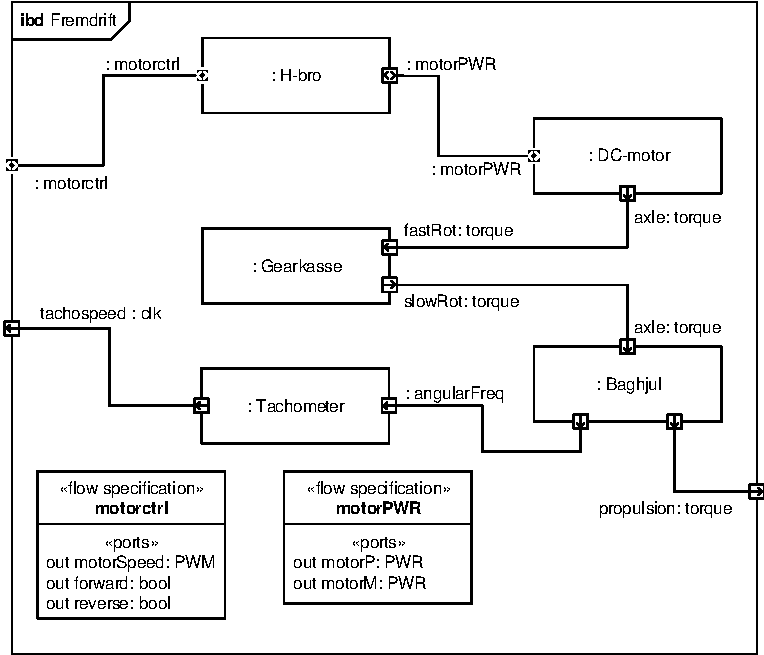
\includegraphics[scale=1]{../fig/diagrammer/bil/ibd_fremdrift.pdf}
\caption{IBD for blokken fremdrift}
\label{fig:ibd_fremdrift}
\end{figure}

\clearpage

\subsubsection{Signalbeskrivelse for fremdrift}

\begin{table}[h]
	\centering
	\begin{tabularx}{\textwidth}{|l|X|X|X|} \hline
	\textbf{Signal (navn: type)} & \textbf{Funktion} & \textbf{Tolerancer} & \textbf{Kommentarer} \\ \hline
motorSpeed: PWM
	& Et PWM signal der bestemmer motorhastigheden. 
	& Frekvens: 30kHz +/- 1kHz 0-5V +/- 0.2V
 	& Logisk signal: \newline
		Lav = 0V +/- 0.2V \newline
		Høj = 5V +/- 0.2V
	\\ \hline

forward: bool
	& Kontrolsignal til H-bro.
	& 0-5V $\pm$ 0.2V
	& Lav = 0V +/- 0.2V  ’idle’ \newline
		Høj =  5V +/- 0.2V  ’frem’
	\\ \hline
	
reverse: bool
	& Kontrolsignal til H-bro.
	& 0-5V $\pm$ 0.2V
	& Lav = 0V +/- 0.2V ’idle’ \newline
		Høj =  5V +/- 0.2V  ’tilbage’
	\\ \hline
	
motorP: PWR
	& Et PWM med frekvens som motorSpeed, dog med mulighed for højere effekt. Dette signal forsyner motoren.
	& Frekvens: 30kHz +/- 1kHz 0-7,2V +/- 0.5V

 	& Logisk signal: \newline
		Lav = 0V +/- 0.5V \newline 
		Høj = 7,2V +/- 0.5V
	\\ \hline

motorM: PWR
	& Reference til motorP.
	& 0V $\pm$ 0.5V
	& ~
	\\ \hline
	
fastRot: torque
	& Kraft der overføres fra motor til gearkasse via drivaksel.
	& - 
	& ~
	\\ \hline
	
slowRot: torque
	& Kraft der overføres fra gearkasse til baghjul via drivaksel.
	& - 
	& ~
	\\ \hline
	
: angularFreq
	& Hjulenes omdrejningshastighed.
	& - 
	& ~
	\\ \hline
	
tachoSpeed: freq
	& Digitalt signal med varierende frekvens afhængig af baghjulenes 					omdrejningshastighed.
	& - 
	& Vejledende: \newline
		64Hz = 10Km/t \newline
		Logisk signal: \newline
		Lav = 0V +/- 0.2V \newline
		Høj = 5V +/- 0.2V

	\\ \hline
	
Propulsion: torque
	& Baghjulenes torque til underlaget.
	& - 
	& ~
	\\ \hline
	\end{tabularx}
\end{table}
\clearpage
\subsection{Styretøj}

De interne signaler for blokken styretøj er beskrevet nedenfor i figur \ref{fig:ibd_styretoej}.

\begin{figure}[h]
\centering
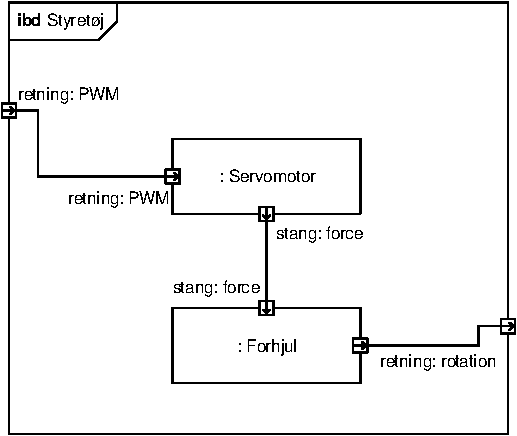
\includegraphics[scale=1]{../fig/diagrammer/bil/ibd_styretoej.pdf}
\caption{IBD for blokken styretøj}
\label{fig:ibd_styretoej}
\end{figure}

\subsubsection{signalbeskrivelse for styretøj}

\begin{table}[h]
	\centering
	\begin{tabularx}{\textwidth}{|l|Z|Z|Z|} \hline
	\textbf{Signal (navn: type)} & \textbf{Funktion} & \textbf{Tolerancer} & \textbf{Kommentarer} \\ \hline
retning: PWM 
	& PWM signal der vha pulsbredden angiver hvilken retning servomotoren skal dreje og dermed hvilken retning bilen skal dreje. 
	& Pulsbredde: 0.5ms – 2.5ms \newline
		Freq = 360Hz \newline
		0.5ms = 18\% Duty cycle (Venstre)\newline
		2.5ms = 90\% Duty cycle (Højre)
	& ~
	\\ \hline
stang: force 
	& Skal overføre kraften fra servomotoren til forhjulene. Dette sker via en stang.
	& -
	& ~
	\\ \hline
retning: rotation
	& Får bilen til at dreje.
	& 30 grader til hhv. venstre og højre $\pm$ 5 grader
	& ~
	\\ \hline
	\end{tabularx}
\end{table}
\clearpage
\subsection{Pi}

Her beskrives intern kommunikation for controlleren Pi i systemet. 

\begin{figure}[h]
\centering
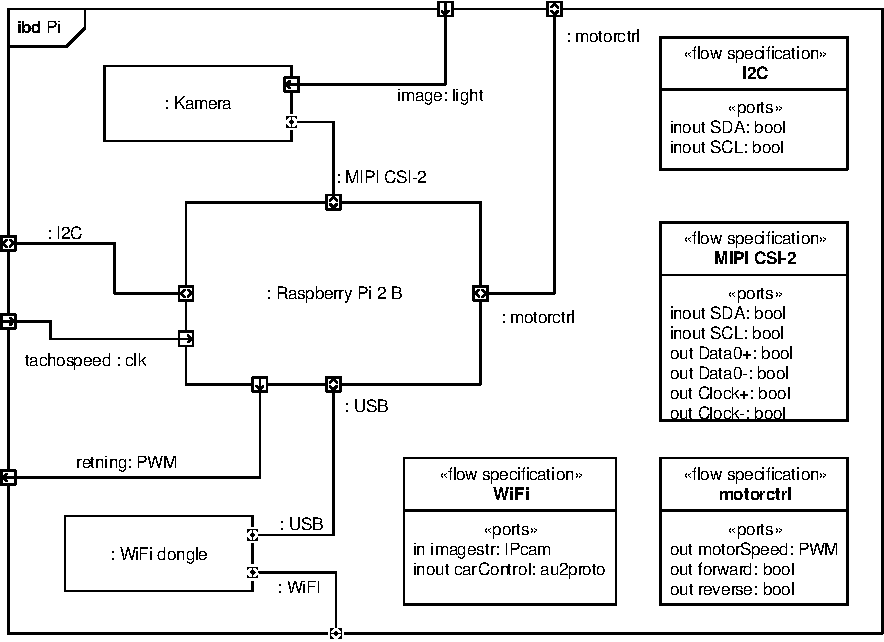
\includegraphics[scale=1]{../fig/diagrammer/bil/ibd_pi.pdf}
\caption{IBD for blokken Pi}
\label{fig:ibd_pi}
\end{figure}
\clearpage


\subsubsection{Signalbeskrivelse for Pi}

\begin{table}[h]
	\centering
	\begin{tabularx}{\textwidth}{|l|Z|Z|Z|} \hline
	\textbf{Signal (navn: type)} & \textbf{Funktion} & \textbf{Tolerancer} & \textbf{Kommentarer} \\ \hline
SDA: bool
	& I2C dataline til sensorer herunder accelerometer og afstandssensorer  
	& 0-5V$\pm$0.5V 
 	& Logisk signal: 			\newline
		Lav= 0V$\pm$0.5V  	\newline
		Høj= 7.2V$\pm$0.5V
	\\ \hline
	
SCL: bool
	& I2C clockline  til sensorer herunder accelerometer og afstandssensorer
	& 0-5V$\pm$0.5V
	& Logisk signal:			\newline 
		Lav= 0V$\pm$0.5V 	\newline
		Høj= 7.2V$\pm$0.5V
	\\ \hline
	
Image: light
	& Lysindfald til kamerasensor
	& -
	& -
	\\ \hline

motorSpeed: PWM	
	& Et PWM signal der bestemmer motorhastigheden.	
	& Frekvens: 30kHz$\pm$1kHz \newline
	  0-5V$\pm$0.2V	
	& Logisk signal: 			\newline 
		Lav= 0V$\pm$0.2V 	\newline
		Høj= 5V$\pm$0.2V
	\\ \hline
	
forward: bool	
	& Kontrolsignal til H-bro
	& 0-5V$\pm$0.2V
	& Logisk signal:					\newline 
		Lav= 0V$\pm$0.2V  ''idle''		\newline
		Høj= 5V$\pm$0.2V  ''forward''
	\\ \hline
	
reverse: bool	
	& Kontrolsignal til H-bro
	& 0-5V$\pm$0.2V	
	& Logisk signal: 					\newline
		Lav= 0V$\pm$0.2V ''idle''		\newline
		Høj= 5V$\pm$0.2V ''back''
	\\ \hline
	
:USB 	
	& Serielforbindelse mellem Wi-fi dongle og Pi	
	& VBUS = 5V$\pm$0.2V 				\newline 
	  D$-$ = 5V$\pm$0.2V				\newline
	  D$+$ = 5V$\pm$0.2V				\newline
	  GND = 0V							\newline	  
	  & VBUS for Low-power port: 		\newline
		Diff  ''1''						\newline
		(D$+$)-(D$-$) > 200 mV			\newline
		og D$+$>VIH (min)				\newline

		Diff ''0''						\newline
		(D$-$)-(D$+$) > 200 mV			\newline
		og D$-$>VIH (min)				\newline
	\\ \hline	
	
imagestr: IPcam
	& At streame video fra kameraet påmonteret på bilen til PC'en.
	& \textit{Ikke angivet} 
	& Laves med 3. parts software	
	\\ \hline

carControl: au2proto
	& At sende data til og fra PC'en til bilen.
	& \textit{Ikke angivet} 
	& ~
	\\ \hline
	
: MIPI CSI-2
	& Kamera serielt interface
	& \textit{Ikke angivet} 
	& Se reference: \cite{lib:MIPICSI-2}
	\\ \hline
	\end{tabularx}
\end{table}

\clearpage
\subsection{Sensorer}

På figur \ref{fig:ibd_sensorer} ses de interne signaler for blokken PI.

\begin{figure}[h]
\centering
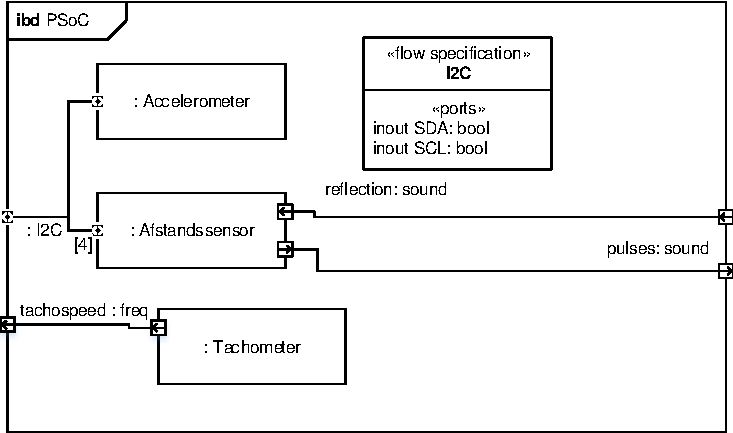
\includegraphics[scale=1]{../fig/diagrammer/bil/ibd_sensorer.pdf}
\caption{IBD for blokken sensorer}
\label{fig:ibd_sensorer}
\end{figure}

\subsubsection{signalbeskrivelse for sensorer}

\begin{table}[h]
	\centering
	\begin{tabularx}{\textwidth}{|l|X|X|X|} \hline
	\textbf{Signal (navn: type)} & \textbf{Funktion} & \textbf{Tolerancer} & \textbf{Kommentarer} \\ \hline
Inout SDA: bool
	& \IIC dataline til sensorer herunder accelerometer og afstandssensorer. 
	& 0-5V $\pm$ 0.5V
 	& Logisk signal: \newline
		Lav = 0V $\pm$ 0.5V \newline
		Høj = 7.2V $\pm$ 0.5V
	\\ \hline

Inout SCL: bool
	& \IIC clockline  til sensorer herunder accelerometer og afstandssensorer. 
	& 0-5V $\pm$ 0.5V
 	& Logisk signal: \newline
		Lav = 0V $\pm$ 0.5V \newline
		Høj = 7.2V $\pm$ 0.5V
	\\ \hline

Pulses: sound
	& Ultralydsbølger afsendt af sensor. 
	& Jfv. Datablad (henvisning kommer senere) %TODO henvsining
 	& ~
	\\ \hline
	
reflection: sound
	& Refleksionsbølge af udsendte ultralydsbølger. 
	& Jfv. Datablad (henvisning kommer senere) %TODO henvsining
 	& ~
	\\ \hline
	\end{tabularx}
\end{table}
\clearpage
\subsection{MPU-6050 Accelerometer/Gyroskop}

MPU-6050 er en kombination af et accelerometer, et gyroskop, begge med 3 akser og et termometer. Det betyder for systemet at det er i stand til at registrere en ændring i acceleration og/eller orientering i alle retninger. Sensoren er blevet valgt til projektet på baggrund af et \IIC interface, som derved kan tilkobles en samlet bus sammen med andre sensorer på bilen. Udover dette giver det konstruerede breakoutboard mulighed for nem tilslutning, men fortsat lille størrelse på sensoren.
Sensoren fungerer altid som en slave med adressen $0b110100X$, hvor X bliver bestemt af det logiske niveau på pin AD0, der som standard er lav. 

\begin{figure}[h]
	\centering
	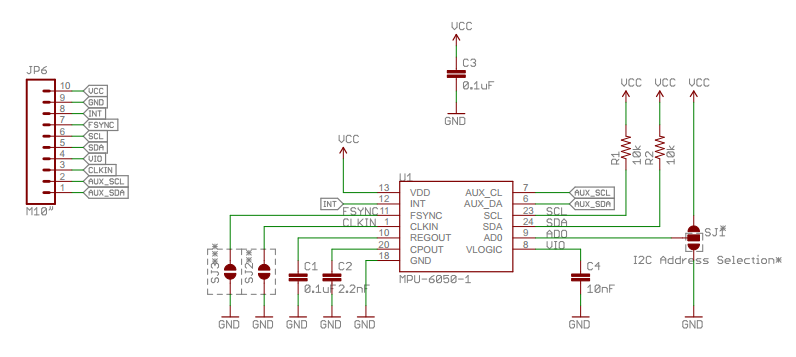
\includegraphics[scale=0.7]{../fig/billeder/mpu6050.png}
	\caption{MPU-6050 diagram}
	\label{fig:mpu6050}
\end{figure}

Diagrammet for sensoren er vist i figur \ref{fig:mpu6050}. Maksimal bushastighed for MPU-6050 er 400kHz, men da der er andre sensorer som arbejder langsommere end MPU-6050 i systemet, passer den fint ind. Accelerometeret er en MEMS-type, hvor der er bygget mikroskopiske kondensatorer ind i chippen, som kan fjedre og bevæge sig, hvilket registreres som en ændring i kapacitans. Denne ændring kan omregnes til nogle brugbare værdier, og kan herfra anvendes til bl.a. retningsbestemmelse. Der er i alt 7 16-bits registre i sensoren, som hver især er tilknyttet til en ADC på hver akse, med undtagelse af register nr. 7, som er tilknyttet termometeret. 
Protokollen for kommunikation med sensoren ser således ud:

\begin{figure}[h]
	\centering
	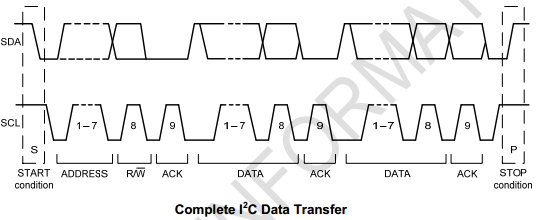
\includegraphics[scale=0.8]{../fig/billeder/mpu6050i2c.png}
	\caption{\IIC protokol for MPU-6050}
	\label{fig:mpu6050i2c}
\end{figure}

Som det ses i figur \ref{fig:mpu6050i2c}, starter masteren med at sætte en startsekvens ud på SDA (HIGH-to-LOW), mens SCL er høj. Herefter betragtes bussen som optaget, indtil der bliver sendt en stopsekvens på SDA (LOW-to-HIGH) af masteren, mens SCL ligeledes er høj. Efter startsekvensen bliver der sendt en 7-bits adresse og en R/W bit. Data der bliver transmitteret over \IIC bliver sendt i pakker af 8 bits. Når der først er sendt en startsekvens, er der ingen begrænsning på hvor meget data der må sendes, udover at der efter hver pakke, skal registreres en acknowledge. MPU-6050 indeholder desuden en DMP (Digital Motion Processor), som har til opgave at håndtere noget af dataprocesseringen fra selve MPU-6050. 

\clearpage
\section{Psoc (PSoC)} \label{sub:sw_impl_psoc_psoc}
\subsection{Psoc (PSoC)}
PSoC'ens formål er at simplificere alt \IIC kommunikation, hvilket viste sig at være en nødvendighed, da implementeringen på Pi'en gav uforudsete problemer med kommunikationen med distancesensorerne.
Da der på Pi'en kører en Linux-distribution foregår \IIC kommunikationen som skrivning og læsning til og fra device-files der repræsenterer de respektive pins (SDA \& SCL), og da kommunikationen med distancesensorerne følger følgende protokollen fra Hardwaredesign afsnittet for distancesensoren.
Ydermere viste det sig at tachometeret, der vha. en schmittrigger trækkes til stel hver gang der detekteres en magnet, dette bliver detekteret som logisk lav på PSoC'en og  kalder den implementerede interrupt service rutine \texttt{ISR}. 
Det vil optage udnødvendig meget af Pi'ens processor og vil være meget tidskritisk i forhold til de andre opgaver som Pi-programmet varetager. Derfor beslutning om at ændre designretning.

Kravet til PSoC'en er, at koden der ligger herpå skal være så hurtig og effektiv som muligt, således at den kan aflæses når PI'en spørger på ny data. 
I listing \ref{lst:getDistance_FL2} ses implementeringen af denne kode.

\lstinputlisting
	[linerange=getDistance::FL-getDistance::FL1, caption=]
	{../../src/psoc/psoc_bil_1/psoc_bil.cydsn/main.c}

\lstinputlisting
	[linerange=getDistance::FL2-getDistance::FL3, label=lst:getDistance_FL2, caption=Front Left sensor aflæsningscyklus.]
	{../../src/psoc/psoc_bil_1/psoc_bil.cydsn/main.c}
	
aflæsningscyklus for de enkelte sensorer er identiske blot med ændret navn og index i \texttt{sendBuffer}

Tachometeret er simplere at aflæse, da alt dataen i forvejen er placeret på PSoC'en. I listing \ref{lst:sw_impl_psoc_getVelocity} ses interrupt service rutinen som køres hver gang der detekteres en magnet på hallswitchen.

\lstinputlisting
	[linerange=getVelocity::1-getVelocity::2, label=lst:sw_impl_psoc_getVelocity, caption=ISR til getVelocity.]
	{../../src/psoc/psoc_bil_1/psoc_bil.cydsn/main.c}

Til sidst kan implementeringen af programmets \texttt{main}-funktion ses i listing \ref{lst:sw_impl_psoc_main}

\lstinputlisting[linerange=main::1-main::2, label=lst:sw_impl_psoc_main, caption=Main program på PSoC.]{../../src/psoc/psoc_bil_1/psoc_bil.cydsn/main.c}

\clearpage

\subsection{Modultest for PSoC}

For at teste om kommunikationen imellem distancesensorene og PSoC'en fungerer korrekt, blev der foretaget en modultest, hvor følgende ønskedes opfyldt. 

\begin{enumerate}
  \item at der kan skrives korrekte kommander til alle 4 sensorer.
  \item at der kan læses korrekte 2-bytes værdier fra alle 4 sensorer.
\end{enumerate}

Der afvikles et main\_test program hvor der kontinuerligt skrives til de 4 sensorer én for én, og derefter læses den nuværende værdi retur i 2-bytes format. 

På figur \ref{fig:write_FL} til \ref{fig:write_RR} ses \texttt{write}-kommando sendt til alle 4 sensorer: 

\begin{figure}[h]
	\centering
	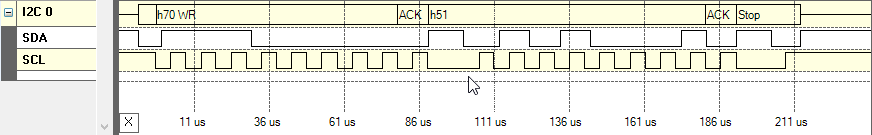
\includegraphics[scale=0.6]{../fig/billeder/psoc_distancesensor_modultest/I2C_write_0x70_FL.png}
	\caption{write til adresse 0x70 sensor FL}
	\label{fig:write_FL}
\end{figure}

\begin{figure}[h]
	\centering
	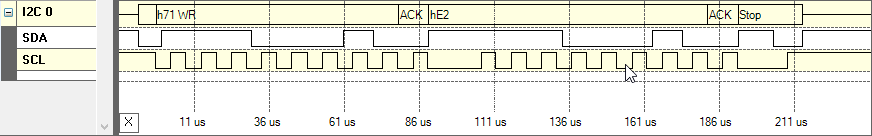
\includegraphics[scale=0.6]{../fig/billeder/psoc_distancesensor_modultest/I2C_write_0x71_FR.png}
	\caption{write til adresse 0x71 sensor FR}
	\label{fig:write_FR}
\end{figure}

\begin{figure}[h]
	\centering
	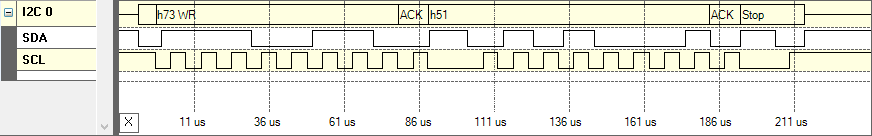
\includegraphics[scale=0.6]{../fig/billeder/psoc_distancesensor_modultest/I2C_write_0x73_RL.png}
	\caption{write til adresse 0x73 sensor RL}
	\label{fig:write_RL}
\end{figure}

\begin{figure}[h]
	\centering
	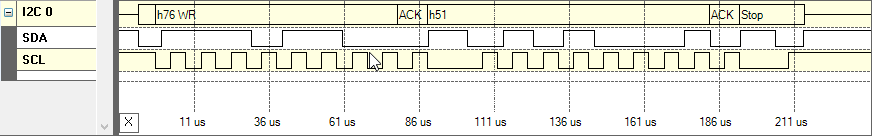
\includegraphics[scale=0.6]{../fig/billeder/psoc_distancesensor_modultest/I2C_write_0x76_RR.png}
	\caption{write til adresse 0x76 sensor RR}
	\label{fig:write_RR}
\end{figure}

\newpage

På figur \ref{fig:read_FL} til \ref{fig:read_RR} ses \texttt{read}-kommando sendt til alle 4 sensorer:

\begin{figure}[h]
	\centering
	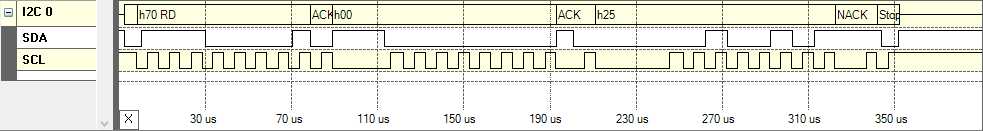
\includegraphics[scale=0.6]{../fig/billeder/psoc_distancesensor_modultest/I2C_read_0x70_FL.png}
	\caption{read til adresse 0x70 sensor FL}
	\label{fig:read_FL}
\end{figure}

\begin{figure}[h]
	\centering
	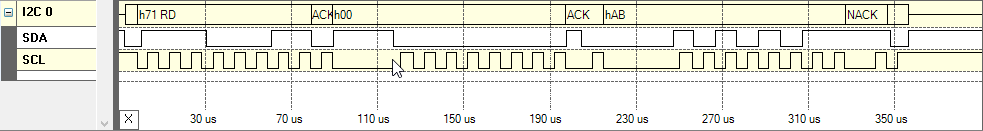
\includegraphics[scale=0.6]{../fig/billeder/psoc_distancesensor_modultest/I2C_read_0x71_FR.png}
	\caption{read til adresse 0x71 sensor FR}
	\label{fig:read_FR}
\end{figure}

\begin{figure}[h]
	\centering
	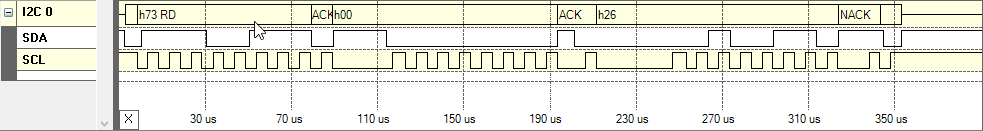
\includegraphics[scale=0.6]{../fig/billeder/psoc_distancesensor_modultest/I2C_read_0x73_RL.png}
	\caption{read til adresse 0x73 sensor RL}
	\label{fig:read_RL}
\end{figure}

\begin{figure}[h]
	\centering
	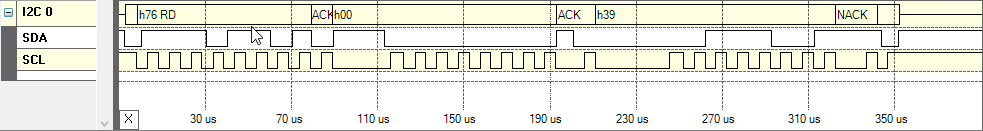
\includegraphics[scale=0.6]{../fig/billeder/psoc_distancesensor_modultest/I2C_read_0x76_RR.png}
	\caption{read til adresse 0x76 sensor RR}
	\label{fig:read_RR}
\end{figure}

\clearpage
\section{Pc}
\subsection{GUI}
\begin{figure}[H]
\centering
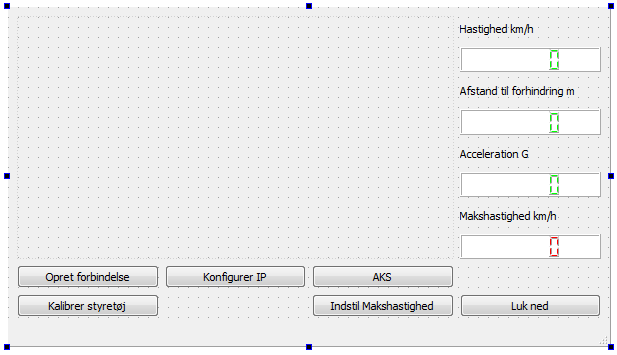
\includegraphics[width=\textwidth* 3/4,height=\textwidth* 9/20 ]{../fig/billeder/gui_design.png}
\caption{GUI i implementerings processen}
\label{fig:GUI_design}
\end{figure}
I denne sektion beskrives funktionerne i \texttt{MainWindow} i detaljer. Udviklingsmiljøet som hele GUI'en er skrevet i er Qt version 5.5 \cite{lib:qt}. En af fordelene ved QT er at man kan lave den grafiske del af GUI'en hurtigt og uden at skulle vide noget om hvordan koden bagved fungerer. Princippet er drag and drop og fungerer ved at man trækker de forskellige knapper og bokse ind i vinduet. Se figur \ref{fig:GUI_design}.
\subsubsection{MainWindow::MainWindow}
Qt opretter selv en klasse kaldet \texttt{MainWindow}. I main funktionen oprettes en instans af \texttt{MainWindow} som gør at hele programmet køres i MainWindow's constructor. Når programmet kører og der trykkes på en knap gives der et signal. Signalet forbindes til et slot i \texttt{constructoren} ved hjælp af funktionen \texttt{connect}. Hovedvinduets \texttt{signals and slots} forbindes i \texttt{constructoren}. I listing \ref{lst:constructor} ses fx. at når der klikkes på \texttt{OpretForbindelse} kaldes funktionen \texttt{Au2connect} som er funktionen der opretter forbindelsen til bilen. Det ses også at variablerne sættes til en default værdi samt der oprettes instanser af VLC-player når \texttt{constructoren} eksekveres. 
\begin{lstlisting}[caption={MainWindows constructor},label=lst:constructor, language=c++]
MainWindow::MainWindow(QWidget *parent)
    : QMainWindow(parent), ui(new Ui::MainWindow),media(0)
{
    isConnected=false;
    controllerConnected=false;
    ui->setupUi(this);
    this->setWindowTitle("Au2");

    instance = new VlcInstance(VlcCommon::args(), this);
    player = new VlcMediaPlayer(instance);
    player->setVideoWidget(ui->video);

    readDataFromFile();

    data[1] = 0;//hastighed
    data[2] = 0;//afstand
    data[3] = 0;//acceleration
    data[4] = 1;//AKS = on

    ui->AKS->setText("AKS-On");

    updateData();
    // Forbindelse af signals og slots 
    connect(ui->OpretForbindelse, SIGNAL(clicked()), this, SLOT(Au2connect()));
    connect(ui->KonfigurerIP, SIGNAL(clicked()), this, SLOT(konfigurerIP()));
    connect(ui->AKS, SIGNAL(clicked()), this, SLOT(AKSstatus()));
    connect(ui->IndstilMaksHastighed, SIGNAL(clicked()), this, SLOT(maksHastighed()));
    connect(ui->KalibrerStyretoj, SIGNAL(clicked()), this, SLOT(kalibrerStyretoj()));
    connect(ui->LukNed, SIGNAL(clicked()), this, SLOT(shutDown()));
    connect(this, SIGNAL(sig_getData()), this, SLOT(readSocket()));
}
\end{lstlisting}
\subsubsection{void MainWindow::Au2connect()}
Når \texttt{Au2connect} bliver kaldt testes der først om forbindelsen allerede er oprettet ved hjælp af variablen \texttt{isConnected}. Er forbindelsen allerede oprettet vil denne variabel være \textbf{true} og der gives besked til brugeren ved hjælp af en messageBox om at forbindelsen allerede er oprettet. Er forbindelsen ikke oprettet, oprettes \texttt{dataSocket} og \texttt{signals and slots} forbindes således signalet \texttt{connected} forbindes til funktionen \texttt{connected}, som sætter variablen \texttt{isConnected} til true samt skaber en messageBox hvor brugeren gives besked om at forbindelsen er oprettet. Derefter oprettes der forbindelse til bilen og der ventes indtil at forbindelsen er etableret, bliver forbindelsen ikke etableret oprettes en messageBox hvori bruger gives besked herom. Lykkedes det at oprette forbindelse kaldes funktionen \texttt{controller} som sørger for at forbinde controlleren med bilen. Når funktionen \texttt{controller} er returneret oprettes dataThread.
\begin{lstlisting}[caption={Au2Connect},label=lst:au2connect, language=c++]
void MainWindow::Au2connect()
{
    if(isConnected)
    {
        QMessageBox messageBox;
        messageBox.information(0,"Status","Forbindelsen er allerede oprettet!");
        messageBox.setFixedSize(500,200);
    }
    else
    {
        socket = new QTcpSocket(this);

        connect(socket,SIGNAL(connected()),this,SLOT(connected()),Qt::DirectConnection);
        connect(socket,SIGNAL(disconnected()),this,SLOT(connectionLost()),Qt::DirectConnection);

        socket->connectToHost(IP,1234);

        if(!socket->waitForConnected(1000))
        {
            QMessageBox messageBox;
            messageBox.critical(0,"Fejl","Forbindelsen blev ikke oprettet!");
            messageBox.setFixedSize(500,200);
        }
        else
        {
            controller();
            int error = pthread_create(&dataThread, NULL, this->getDataHelper ,this);
               if(error !=0)
              {
                qDebug()<<"Error on pthread_create"<<endl;
                return;
              }

            openPlayer();
         }
     }
}
\end{lstlisting}
\subsubsection{void MainWindow::controller()}
Funktionen \texttt{controller()} sørger for at forbinde controlleren med bilen. Der oprettes først en instance af \texttt{Xboxcontroller} hvorefter der testes om controlleren er forbundet. Er controlleren ikke forbundet oprettes der en messageBox hvori brugeren gives besked herom. Hvis controlleren er forbundet oprettes \texttt{controllerSocket} og dens \texttt{signals and slots} forbindes. Efterfølgende skabes der forbindelse og der testes om det lykkedes. Lykkedes det ikke gives bruger besked herom. Ellers oprettes \texttt{controllerThread} og funktionen returnerer. Se Listing \ref{lst:controller}.
\begin{lstlisting}[caption={controller},label=lst:controller, language=c++]
void MainWindow::controller()
{

    XboxController_ = new XboxController(1);

    if(!XboxController_->connect())
    {
        QMessageBox messageBox;
        messageBox.critical(0,"Fejl","Controlleren er ikke tilsluttet");
        messageBox.setFixedSize(500,200);
        delete XboxController_;
        return;
    }

    controllerSocket = new QTcpSocket;

    connect(controllerSocket,SIGNAL(connected()),this,SLOT(controllerIsConnected()),Qt::AutoConnection);
    connect(controllerSocket,SIGNAL(disconnected()),this,SLOT(controllerLostConnection()),Qt::AutoConnection);

    controllerSocket->connectToHost(IP,1235);

    if(!controllerSocket->waitForConnected(1000))
    {
        QMessageBox messageBox;
        messageBox.critical(0,"Fejl","Controlleren kunne ikke oprette forbindelse til bilen");
        messageBox.setFixedSize(500,200);
        delete controllerSocket;
        delete XboxController_;
    }
    else
    {
        int error = pthread_create(&controllerThread, NULL, this->controllerStreamHelper ,this);
           if(error !=0)
          {
            qDebug()<<"Error on pthread_create controller"<<endl;
            return;
          }

     }

}
\end{lstlisting}
\subsubsection{void* MainWindow::controllerStream()}
Funktionen \texttt{controllerStream()} streamer data fra controlleren til bilen således bilen kan reagere på input fra brugeren. Funktionen starter med at oprette et array hvori controller data gemmes. Data fra \texttt{XboxController} hentes og sendes til bilen ved hjælp af \texttt{controllerSocket} i en while-løkke, så længe \texttt{controllerConnected} er \textbf{true}.
\begin{lstlisting}[caption={controllerStream},label=lst:controller, language=c++]
void* MainWindow::controllerStream(void)
{
    char controllerData[4]={0};
    char turn;
    unsigned char forward;
    unsigned char back;
    bool brake;
    while (controllerConnected)
    {
        XboxController_->getCtrData(turn, forward, back, brake);
        controllerData[0]=forward;
        controllerData[1]=back;
        controllerData[2]=turn;
        controllerData[3]=(char)brake;
        controllerSocket->write(controllerData,4);
        controllerSocket->waitForBytesWritten();
        QThread::msleep(10);
    }

    return NULL;
}
\end{lstlisting}
\subsubsection{void* MainWindow::controllerStreamHelper()}
Funktionen \texttt{controllerStreamHelper} kaldes når \texttt{controllerThread} oprettes af \texttt{p\_thread\_create}. Da \texttt{p\_thread\_create} kun kan tilgå \texttt{static} funktioner gøres \texttt{controllerStreamHelper} \texttt{static} i \texttt{MainWindow.h}. Funktionen returnerer blot en pointer til \texttt{controllerStream}
\begin{lstlisting}[caption={controllerStream},label=lst:controller, language=c++]
void* MainWindow::controllerStreamHelper(void* context)
{
    return ((MainWindow *)context)->controllerStream();
}
\end{lstlisting}

\subsubsection{void* MainWindow::getData()}
Funktionen \texttt{getData} kører i en while-løkke så længe variablen \texttt{isConnected} er true. \texttt{isConnected} sættes til \textbf{true} når \texttt{dataSocket} har oprettet forbindelsen til bilen og false når \texttt{dataSocket} mister forbindelsen. I while-løkken gives signalet \texttt{sig\_getData} som gør at \texttt{MainWindow} eksekverer funktionen \texttt{readSocket} som sender og henter nyt data fra bilen. Efterfølgende eksekveres funktionen \texttt{updateData} som opdater variablerne i hovedvinduet.
\begin{lstlisting}[caption={getData},label=lst:getData, language=c++]
void* MainWindow::getData(void)
{
    while(isConnected)
    {
        sig_getData();
        updateData();
        QThread::msleep(100);
    }
    return NULL;
}
\end{lstlisting}
\subsubsection{void* MainWindow::getDataHelper()}
Funktionen \texttt{getDataHelper} kaldes når \texttt{dataThread} oprettes af \texttt{p\_thread\_create}. Da \texttt{p\_thread\_create} kun kan tilgå \texttt{static} funktioner gøres \texttt{getDataHelper} \texttt{static} i \texttt{MainWindow.h}. Funktionen retunerer blot en pointer til \texttt{getData}
\begin{lstlisting}[caption={getDataHelper},label=lst:getData, language=c++]
void* MainWindow::getDataHelper(void* context)
{
    return ((MainWindow *)context)->getData();
}
\end{lstlisting}

\subsubsection{void MainWindow::readSocket()}
Funktionen \texttt{readSocket} sender og læser data fra bilen. Når funktionen eksekveres låses \texttt{mutex} således andre funktioner ikke kan tilgå samme data.
\begin{lstlisting}[caption={readSocket},label=lst:readSocket, language=c++]
void MainWindow::readSocket()
{   
    mutex.lock();
    socket->write(data,6);
    socket->waitForBytesWritten();
    socket->waitForReadyRead();
    socket->read(data,6);
    mutex.unlock();
}
\end{lstlisting}

\subsubsection{void MainWindow::konfigurerIP()}
Funktionen \texttt{konfigurerIP} åbner for en inputdialog som giver brugeren mulighed for at indtaste en IP-adressen. IP-adressen gemmes i variablen \texttt{IP} og variablen \texttt{videoUrl} opdateres til stream-adressen fra bilen.
\begin{lstlisting}[caption={konfigurerIP},label=lst:konfigurerIP, language=c++]
void MainWindow::konfigurerIP()
{
    QString copy = IP;
    IP = QInputDialog::getText(this, tr("Konfigurer IP"), tr("Indtast IP adressen"), QLineEdit::Normal,IP);
    if (IP.isEmpty()){
    IP = copy;
    return;
    }
    videoUrl = "http://"+IP+":8081/stream.mjpeg";
}
\end{lstlisting}

\subsubsection{void MainWindow::AKSstatus()}
Funktionen \texttt{AKSstatus} ændre status på AKS på bilen. Når bruger trykker på knappen ''AKS-on'' ændres teksten til ''AKS-off'' og omvendt. Plads 4 i data arrayet opdateres til henholdsvis 1 eller 0. 
\begin{lstlisting}[caption={AKSstatus},label=lst:AKSstatus, language=c++]
void MainWindow::AKSstatus()
{
    data[4] =!data[4];
    if(data[4])
    ui->AKS->setText("AKS-On");
    else
    ui->AKS->setText("AKS-Off");
}
\end{lstlisting}

\subsubsection{void MainWindow::maksHastighed()}
Funktionen \texttt{maksHastighed} åbner en inputdialog hvor bruger gives mulighed for at indtaste en værdi mellem 0 og 10 i intervaller på 1. Alt uden for dette interval blokeres.  
\begin{lstlisting}[caption={maksHastighed},label=lst:maksHastighed, language=c++]
void MainWindow::maksHastighed()
{
    int copy = (int)data[0];
    bool ok;

    data[0] = (char)QInputDialog::getInt(this, tr("Makshastighed"),tr("Indtast makshastigheden"),
                                         (int)data[0], 0, 10, 1, &ok);
    if (!ok)
        data[0] = (char)copy;

    ui->lcdMakshastighed->display((int)data[0]);
}
\end{lstlisting}

\subsubsection{void MainWindow::writeDataToFile()}
Funktionen \texttt{writeDataToFile} åbner logfilen \texttt{Au2Data.txt} og skriver data arrayet til filen. Funktionen kaldes i \texttt{destructoren} således brugerinput gemmes når programmet lukkes. 
\begin{lstlisting}[caption={writeDataToFile},label=lst:writeDataToFile, language=c++]
void MainWindow::writeDataToFile()
{
    QFile file("Au2Data.txt");
        if(!file.open(QIODevice::WriteOnly))
            return;

    QTextStream out(&file);
    out << IP << "\r\n";
    out << videoUrl << "\r\n";
    out << (int)data[5] << "\r\n";
    out << (int)data[0] << "\r\n";
}
\end{lstlisting}

\subsubsection{void MainWindow::readDataFromFile()}
Funktionen \texttt{readDataFromFile} åbner logfilen \texttt{Au2Data.txt} og læser data arrayet fra filen. Funktionen kaldes i \texttt{constructoren} således brugerinput genindlæses ved opstart. 
\begin{lstlisting}[caption={readDataFromFile},label=lst:readDataFromFile, language=c++]
void MainWindow::readDataFromFile()
{
    QFile file("Au2Data.txt");
        if(!file.open(QIODevice::ReadOnly))
            return;

    QTextStream in(&file);
    IP = in.readLine();
    videoUrl = in.readLine();
    data[5] = (char)in.readLine().toInt();
    data[0] = (char)in.readLine().toInt();
}
\end{lstlisting}

\subsubsection{void MainWindow::kalibrerStyretoj()}
Funktionen \texttt{kalibrerStyretoj} åbner en inputdialog som giver brugeren mulighed for at indtaste en værdi mellem -50 og 50. Inputdialogen blokerer selv for værdier uden for dette interval.
\begin{lstlisting}[caption={kalibrerStyretoj},label=lst:kalibrerStyretoj, language=c++]
void MainWindow::kalibrerStyretoj()
{
    int copy = (int)data[5];
    bool ok;

    data[5] = (char)QInputDialog::getInt(this, tr("Styretoj"),tr("Indstil styretoj"),
                                         (int)data[5], -50, 50, 1, &ok);
    if (!ok)
        data[5] = (char)copy;
}
\end{lstlisting}

\subsubsection{void MainWindow::shutDown()}
Funktionen \texttt{shutDown} kaldes når GUI'en lukkes ned, enten i det røde kryds eller på knappen luk ned. Funktionen tester først om \texttt{dataSocket} er forbundet ved hjælp af variablen \texttt{isConnected}. Er der forbindelse låses \texttt{mutex} og der skrives \textbf{''dwnnow''} til bilen. Returneres dette igen fra bilen, har bilen accepteret at lukke ned. Hvis ikke dette modtages, åbnes en advarsel som giver bruger besked herom. Er forbindelsen ikke forbundet kaldes \texttt{MainWindows destructor} med funktionen \texttt{close}. 
\begin{lstlisting}[caption={shutDown},label=lst:shutDown, language=c++]
void MainWindow::shutDown()
{
    if(isConnected)
    {
        char sdata[6];
        mutex.lock();
        socket->write("dwnnow",6);
        socket->waitForBytesWritten();
        socket->waitForReadyRead();
        socket->read(sdata,6);
        if(sdata[0]=='d' && sdata[1]=='w' && sdata[2]=='n' && sdata[3]=='n' && sdata[4]=='o' && sdata[5]=='w')
        {
            socket->disconnect();
            mutex.unlock();
            close();
        }
        else
        {
            mutex.unlock();
            QMessageBox messageBox;
            messageBox.critical(0,"Fejl","Bilen kan ikke lukke ned!\n Prøv igen");
            messageBox.setFixedSize(500,200);
            return;
        }
    }
    close();
}
\end{lstlisting}

\subsubsection{void MainWindow::MainWindow()}
Dette er \texttt{MainWindows destructor} som først kalder \texttt{writeDataToFile} og derefter sletter oprettede instanser.
\begin{lstlisting}[caption={MainWindow},label=lst:MainWindow, language=c++]
MainWindow::~MainWindow()
{
    writeDataToFile();

    if(controllerSocket != NULL)
        delete controllerSocket;

    if(socket != NULL)
        delete socket;

    if(media != NULL)
        delete media;

    delete player;
    delete instance;
    delete ui;
}
\end{lstlisting}

\subsection{VLC}
Udviklingsmiljøet som hele GUI'en er skrevet i er Qt version 5.5. For at inkludere VLC, skal Qt være installeret \cite{lib:qt}. For at kunne modtage video stream i GUI'en skal vi bruge en forbygget version af VLC til windows32 indeholdende .dll filer osv, samt bilioteker til Qt. Dette gøres ved at udpakke Filen \textbf{vlc-2.0.7-win32.7z} som hentes fra en ftp server \cite{lib:vlc-ftp}. til destinationen \textbf{c:/Qt/}. Pakken indeholder rumtime-filerne som senere skal kopieres over i debugfolderen. Include filerne til Qt downloades \textbf{“Official VLC-Qt Windows SDK and Source Packages”} \cite{lib:vlc-qt} og udpakkes i \textbf{c:/Qt/}. I denne pakke ligger der et demoprojekt som der er hentet inspiration fra til projektet. Laves der et nyt projekt skal der inkluderes de rigtige filer til Qt. Dette gøres ved at åbne .pro filen i Qt og tilføje:

\begin{lstlisting}
# Edit below for custom library location
LIBS     += -LC:\Qt\libvlc-qt\lib -lvlc-qt -lvlc-qt-widgets
INCLUDEPATH += C:\Qt\libvlc-qt
\end{lstlisting}
Når projektet er bygget kopieres filerne \textbf{libvlc-qt-widgets.dll} og \textbf{libvlc-qt.dll} fra \textbf{C:/Qt/libvlc-qt/bin} til build folderen. Efterfølgende kopieres filerne \textbf{axvlc.dll, libvlc.dll, libvlccore.dll} og \textbf{npvlc.dll} fra \textbf{C:/Qt/vlc-2.0.7} samt folderen \textbf{plugins} også til buildfolderen. Programmet skulle nu genre kunne køre. Hvis ikke kan der findes mere hjælp her \cite{lib:vlc-using-qt}. Desværre er der nogle fejl i linket, som der gerne skulle være rettet i denne beskrivelse. 
\clearpage

